\section {Shape Detection and Processing}
\label{sec:related_work_shape detection}

The objective of detecting structures in point clouds is a wide field of research. The term structure is defined very loosely. Structure can mean geometric structures, such as planes, cylinders, or spheres. Structure can also be interpreted as more complex components that represent distinct man-made or natural formations, such as cars or lanterns. This thesis draws inspiration from different shape-detection approaches and pairs them with a clustering algorithm to detect relationships between shapes. 

\par

%Hough transform

The 2D Hough transform \cite{hough1962method} is a technique used usually in the field of image processing. This method can detect straight lines such as building contours as well as curves. The Hough transform was extending to 3D by Maas et al. \cite{maas1999two} and later by Oda et al. \cite{oda2004automatic} and Overby et al. \cite{overby2004automatic}. Rabbani et al. \cite{rabbani2005efficient} utilize the 3d Hough transform to detect cylinders as well. 


\begin{figure}
    \centering
    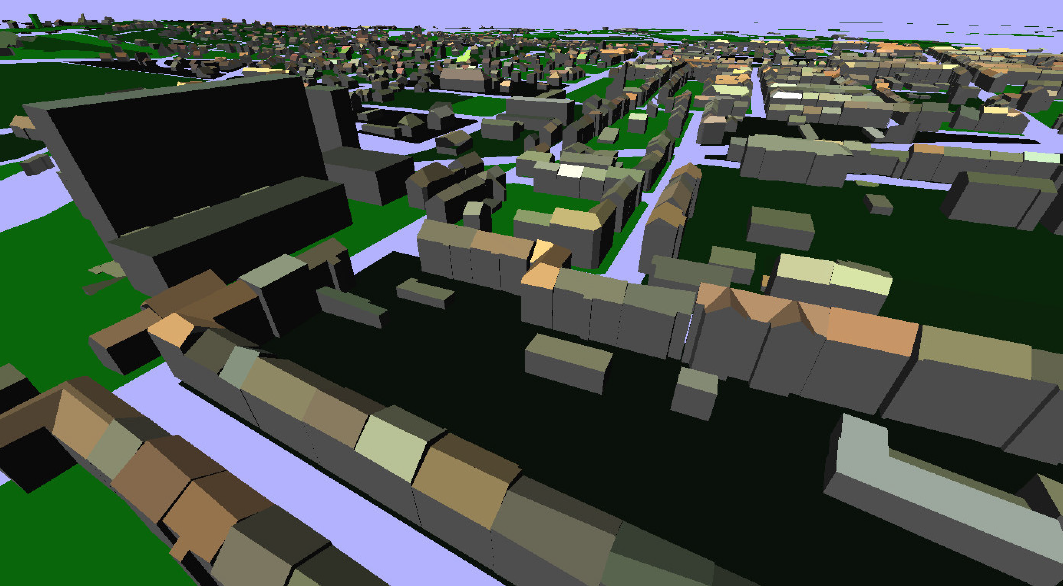
\includegraphics[width=0.81\textwidth]{Related_Work/hough_planes.png}%7
    \caption[Scene created by using 3d Hough transform to detect planes from an airborne laser scanner]
		{Scene created by using 3D Hough transform to detect planes from an airborne laser scanner. Image by Overby et al. \cite{overby2004automatic}.}
    \label{fig:hough_planes}
\end{figure}

Figure \ref{fig:hough_planes} shows a city model consisting of planes, detected using 3D Hough transform, in a point cloud obtained from airborne laser scanning. Figure \ref{fig:hough_cylinder} showcases a point cloud obtained by a 3d scan and the detected cylinders. 


\begin{figure}
\centering
\subcaptionbox{ \label{fig:picking_raycast }}{
  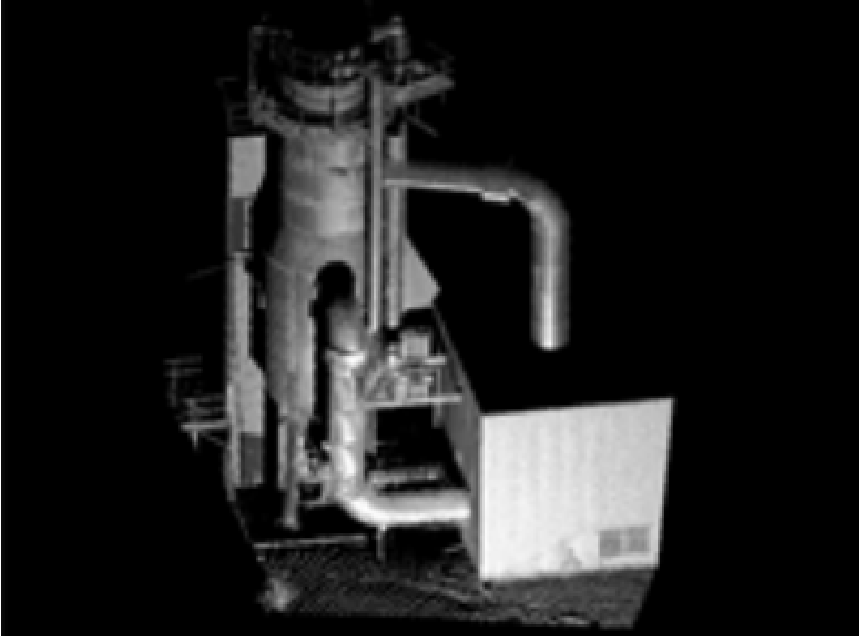
\includegraphics[width=0.4\textwidth]{Related_Work/hough_cylinder1.png}
  }
\subcaptionbox{ \label{fig:picking_conecast }}{
  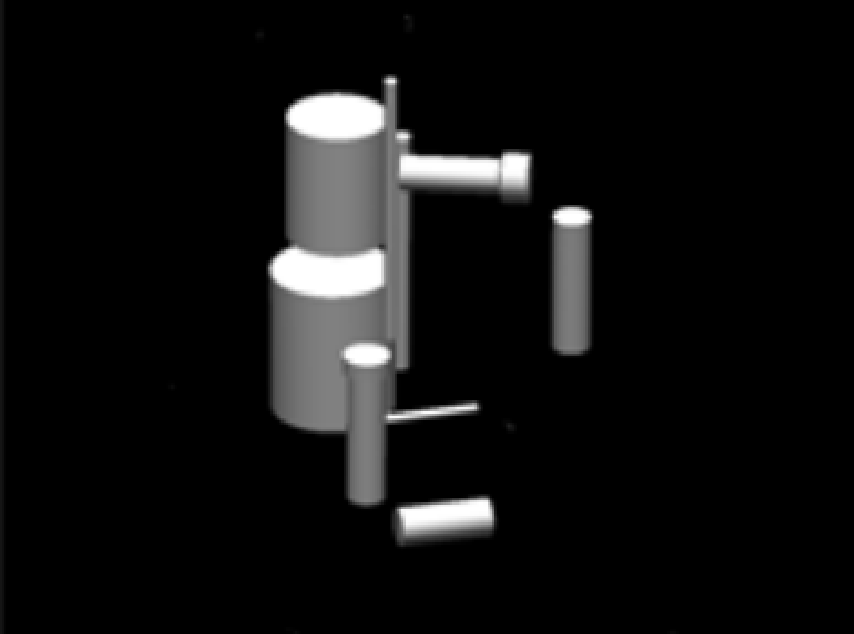
\includegraphics[width=0.4\textwidth]{Related_Work/hough_cylinder2.png}
  }
\caption[Results of 3d Hough transform used to detect cylinders]
{This figure shows the results of the 3D Hough transform for cylinder detection. (a) shows the input point cloud, (b) shows the detected cylinders. Image by Rabbani et al. \cite{rabbani2005efficient}.}
\label{fig:hough_cylinder}
\end{figure}

% Ransac-Based

Schnabel et al. \cite{schnabel-2007-efficient} propose an alternate technique for shape detection. The authors propose the use of Random Sampling Consensus \cite{fischler1981random} to extract a minimal set of primitive shapes that approximate the global structure of the point cloud. The algorithm randomly selects a set of points that roughly follow the curvature of a shape. If a defined number of points are approximated by this shape, the shape is considered to be valid. This approach is capable of detecting planes, cylinders, spheres, cones, and tori and has evolved into one of the most prominent shape detection algorithms and is used in this thesis as well. Later, Schnabel et al. \cite{schnabel-2007-ransac} extended their existing solution, to be capable to process out-of-core datasets. An octree is used that partitions the point cloud into chunks of data that are suitable as input for their RANSAC shape detection. 

\begin{figure}
    \centering
    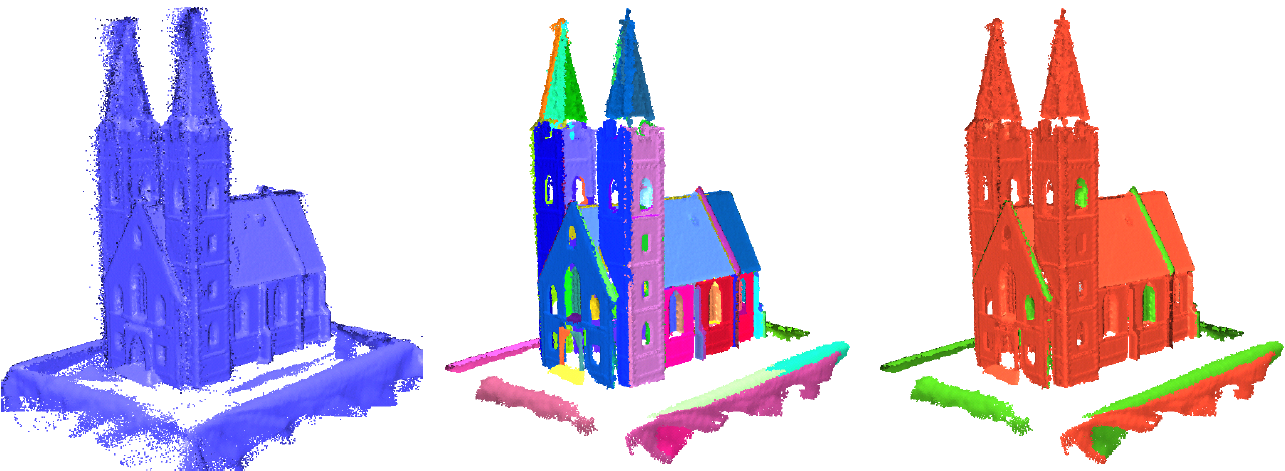
\includegraphics[width=0.8\textwidth]{Related_Work/schnabel_example.png}%7
    \caption[Church with points colored by detected shape]
		{Left: the original point cloud. Center: The points that belong to a detected shape in random colors. Right: The colors are determined by type (plane = red, cylinder = green, sphere = yellow, cone = purple, torus = grey). Image by Schnabel et al. \cite{schnabel-2007-efficient}. }
    \label{fig:schnabel_church}
\end{figure}

Figure \ref{fig:schnabel_church} shows the results of the RANSAC approach on a point cloud. Not only does this approach provide the geometry of the detected shapes, it also determines the membership of a point to a shape. 

\par

Tarsha-Kurdi et al. \cite{tarsha2007hough} analyze the performance of the 3D Hough transform and RANSAC for detecting roof planes from airborne laser data. RANSAC proves to be more robust to noise and more efficient.

\par

Besides the RANSAC approach and the Hough transform, graph-based methods are an alternative approach for shape detection and object recognition. Golvinskiy et al. \cite{golovinskiy2009shape} utilize graph-based methods paired with machine learning to recognize shapes in urban environments in 3D point clouds. This method can detect objects, such as cars, newspaper boxes and traffic lights. Potential object locations are identified by clustering nearby points before the point cloud is segmented into foreground and background. For each cluster, a feature vector is built that is used in a trained classifier to obtain a final classification. By using a pre-trained classifier, any type of object can be detected. This method has the benefit of not being limited to the basic shapes types as with the RANSAC approach. 

\par

Due to manufacturing reasons, man-made objects are often a composition of primitive shapes that follow constraints, such as parallelism and orthogonality. 
While RANSAC and the Hough transform produce satisfactory results, these relations between shapes are often overlooked. Therefore, algorithms that determine relations between shapes and refit the point cloud accordingly are needed to introduce information on a global scale to the point cloud. 
GlobFit by Li et al. \cite{li2011globfit} uses the RANSAC approach to detect primitive shapes along with their global mutual relations. The authors propose an automated approach that iteratively learns from the local relations and adjusts the shape-detection constraints accordingly. Starting from an initial set of RANSAC-detected primitives, the system searches for relations, such as orientation (e.g., parallelism, orthogonality), placement (e.g., coplanarity, coaxis), and equality among shapes and refits the point cloud to match the shapes, before serving as input for the next iteration. 

\par

O-Snap by Arikan et al. \cite{arikan-2013-osn} utilizes Schnabel's algorithm to extract an initial model from a point cloud used in a reconstruction and modeling pipeline. Their approach introducse an additional polygonization step that creates enclosing polygons from detected shapes and approximated points using the local adjancency relations of the point cloud. They combine these automatic steps in an interactive workflow to snap polygon elements together, while simultaneously fitting the input point cloud to ensure the planarity of the polygons. 

\par

Oesau et al. \cite{oesau2016planar} propose an alternative approach to detect planar shapes in point clouds by using region growing and pairs it with a procedure to detect relationsships between shapes. A shape is represented as a set of points and an associated fitting plane. Points or shapes from the neighborhood are added consecutively to the plane, thus growing the region. After shape detection, relationships (regularities) between shapes are determined. First, parallel relationships are detected and the shapes are realigned to a cluster. In a next step, orthogonal relationships between two clusters are determined. Coplanarity relationships are detected by creating a cluster based on the distance between planes. 
